\section{Simulations}
\label{sec:simulations}
Figure \ref{fig:strongARM_out} shows the output of the stongARM latch for alternating data at the input for \unit[6]{UI}. For the simulation a data pattern of 11001100 was feed into the input of the receiver. As we have two slices with half-rate clocking this results in alternating data for one of the slices. To degenerate the signal and take the limited bandwith of the channel into account a RC circuit was used at the receiver input resulting in the \textit{in+} and \textit{in-} signals. The \textit{set} and \textit{reset} signals are the direct outputs of the strongARM circuit and the \textit{RS\_out} signal is one of the RS-FlipFlop outputs.

The frequency response of the variable offset amplifier (VOA) is shown in figure \ref{fig:voa_freq} and its ac noise response is drawn in figure \ref{fig:voa_noise}.

\begin{figure}[H]
  \centering
  {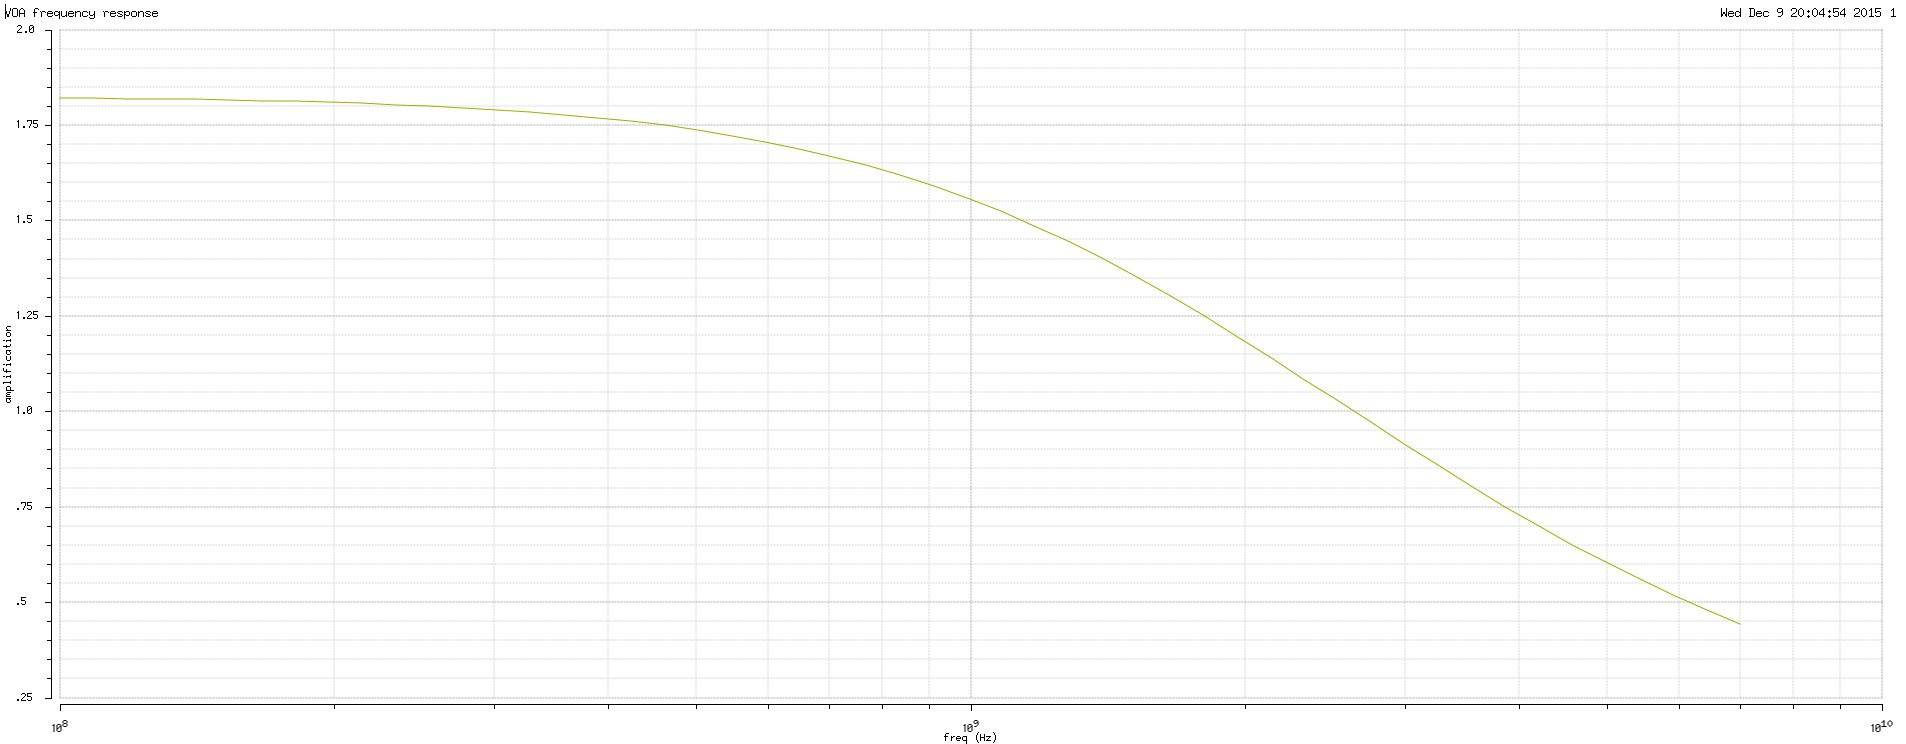
\includegraphics[scale=0.35]{img/voa_freq.jpg}}
  \caption{VOA frequency response}
  \label{fig:voa_freq}
\end{figure}

\begin{figure}[H]
  \centering
  {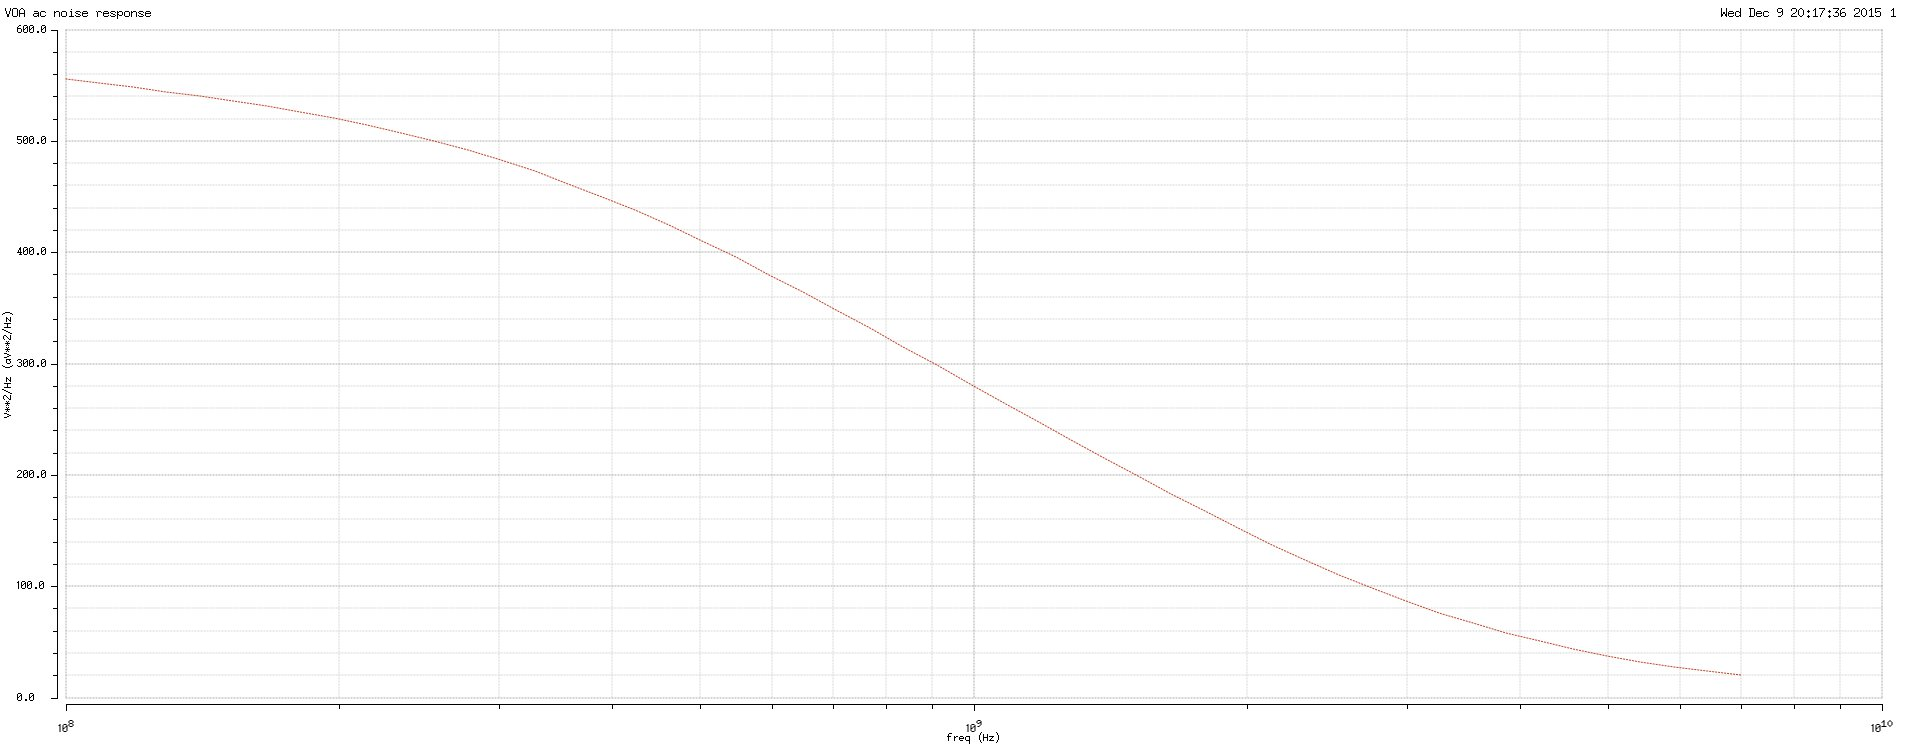
\includegraphics[scale=0.35]{img/voa_noise.jpg}}
  \caption{VOA ac noise response}
  \label{fig:voa_noise}
\end{figure}

\begin{figure}[H]
  \centering
  {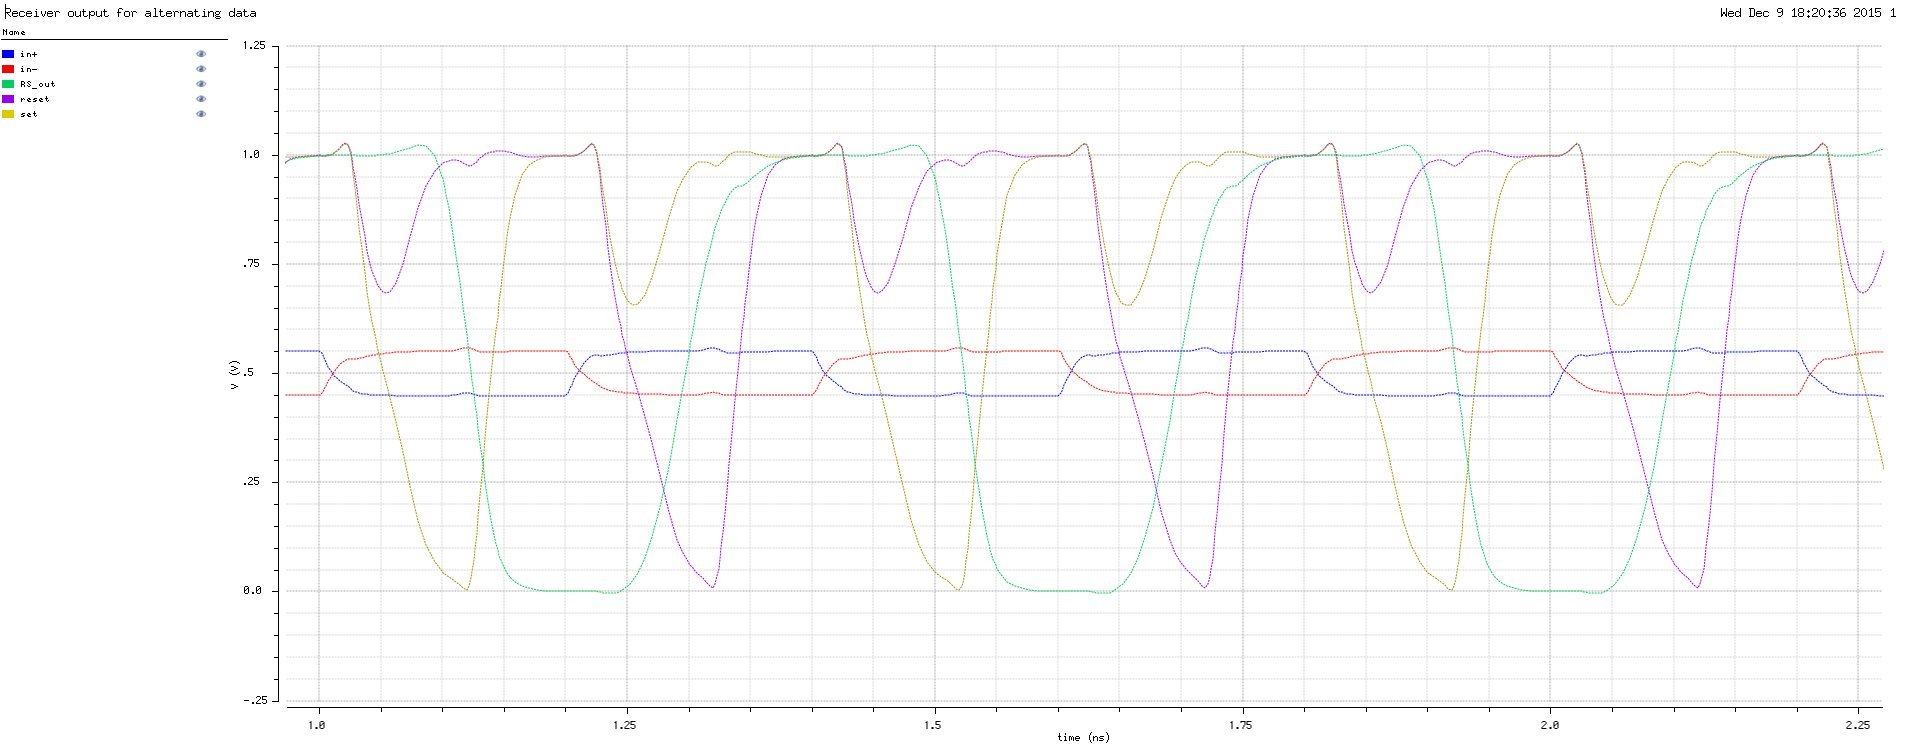
\includegraphics[angle=90, scale=0.45]{img/output_alt_trans.jpg}}
  \caption{Transient waveform for alternating data at the output of the strongARM latch}
  \label{fig:strongARM_out}
\end{figure}